\newcommand{\psd}[1]{{\small\sffamily{\color{blue!60}#1}}}

So far in the previous cases we only concentrated on bar simulations,
which were more or less trivial cases. Moreover, the bar meshes are
provided with the PSD solver. In this section we now turn towards 3D
simulation of a mechanical piece, the geometry of which is shown in
\cref{fig:mechanicalpiecegeo}. The left (small) hole is fixed:
\(u_1=u_2=u_3=0\), while as traction force \(t_x=10^9\) is applied on
the large hole.

You can grab a copy of CAD geometry for the mechanical piece (the Gmsh
\psd{.geo}) your local Gmsh installation folder
\psd{gmsh/share/doc/gmsh/demos/simple\_geo/piece.geo}. To generate the
mesh \psd{piece.msh} simply do

\begin{lstlisting}[style=BashInputStyle]
gmsh -3 piece.geo -format msh2
\end{lstlisting}

Now the PSD simulation can be performed.

\begin{figure}[h]
    \centering
    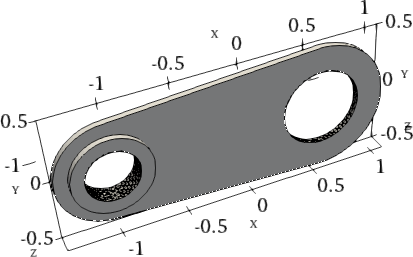
\includegraphics[align=b,width=0.5\textwidth]{./Images/3d-mechanical.png}
    \caption{3D mechanical piece.}
    \label{fig:mechanicalpiecegeo}
\end{figure}

\textbf{Step 1: Preprocessing}

As a prerequiste, place the generated mesh \psd{piece.msh} in any folder
of your choice (assuming you are working in a folder
\psd{psd-complex-simulation}). For ``PSD Preprocessing'' phase, in the
folder \psd{psd-complex-simulation} launch the terminal there and run
the following command.

\begin{lstlisting}[style=BashInputStyle]
PSD_PreProcess  -problem linear-elasticity -dimension 3 -dirichletconditions 1 -tractionconditions 1 -postprocess u
\end{lstlisting}

Here, by using these parameters we have generated one Dirichlet
condition and one traction condition, respectively to be applied to the
small and the large holes in the mesh. Further, by using
\psd{ -dimension 3} we have let PSD know that the problem is 3D .In the
\psd{/PSD/Meshes/3D/piece.msh} generated, the label 4 (resp. 3)
corresponds to the Dirichlet (resp. traction) border. To provide
Dirichlet conditions on label number 4 (\(u_x=0,u_y=0,u_z=0\)) in
\psd{ ControlParameters.edp} use set \psd{Dbc0On 4}, \psd{ Dbc0Ux 0.},
\psd{ Dbc0Uy 0.}, and \psd{ Dbc0Uz 0.}. To add the values and label
numbers of the traction borders edit the \psd{ ControlParameters.edp},
set \psd{ Tbc0On 3} and \psd{ Tbc0Ty -1.e9}. For this end
\(\mathbf t=[t_x,t_y,t_z]=[0.,10^9,0.]\). Finally we use steel
properties for the material, so in \psd{ ControlParameters.edp} the
parameters \psd{ real E  = 200.e9;} and \psd{ real nu = 0.3;} should be
used. These represent \(E\) and \(\nu\), respectively.

\textbf{Step 2: Solving}

Let us now use 2 cores to solve this problem. To do so enter the
following command:

\begin{lstlisting}[style=BashInputStyle]
PSD_Solve -np 2 Main.edp -mesh ./piece.msh
\end{lstlisting}

\textbf{Step 3: Postprocessing}

Launch ParaView and have a look at the \psd{ .pvd} file in the
\psd{ PSD/Solver/VTUs\_DATE\_TIME} folder.

\begin{figure}[htbp]
    \centering
    \begin{minipage}[t][2cm][t]{0.36\textwidth}
    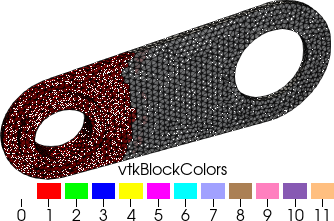
\includegraphics[align=b,width=1\textwidth]{./Images/3d-mechanical-part.png}
    \end{minipage}\hspace{.1\textwidth}
    \begin{minipage}[t][2cm][t]{0.4\textwidth}
    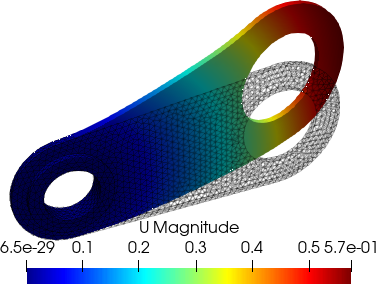
\includegraphics[align=b,width=1\textwidth]{./Images/3d-mechanical-result.png}
    \end{minipage}
    \caption{Mechanical piece test results. Partitioned mesh (left) and  warped displacement field (right).}
    \label{fig:mechapieceresult}
\end{figure}

\textbf{Redoing the test with different conditions}

\begin{figure}[htbp]
    \centering
    \begin{minipage}{0.42\textwidth}
    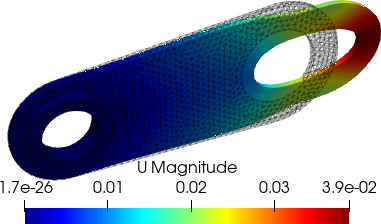
\includegraphics[align=b,width=1\textwidth]{./Images/3d-mechanical-result-x.png}
    \end{minipage}
    \caption{Mechanical piece test results: \psd{ real  tx0=1.e9, ty0=0, tz0=0.,;}}
\end{figure}

\begin{figure}[htbp]
    \centering        
    \begin{minipage}{0.4\textwidth}
    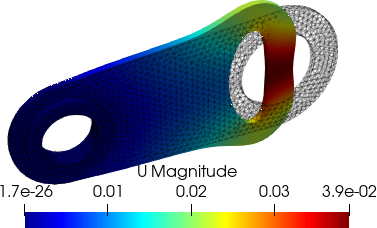
\includegraphics[align=b,width=1\textwidth]{./Images/3d-mechanical-result--x.png}
    \end{minipage}
    \caption{Mechanical piece test results:\psd{ real  tx0=1.e9, ty0=0, tz0=0.,;}}
    \label{fig:mechapieceresult2}
\end{figure}
